\section{Characteristic Functions}
In this chapter, we look at characteristic functions of measures of $(\R^n, \B(\R^n))$, as well as random variables taking value on this measurable space. Let us begin by stating the definition.

\begin{definition}[Characteristic Functions]
\begin{itemize}
\item[]
\item The characteristic function of a measure $\mu$ on $(\R,\B(\R))$ is 
\begin{equation}
    \varphi_\xi(t) := \varphi(t) := \int_{-\infty}^\infty e^{itx} \, \mu(dx), \quad t \in \R.
\end{equation}
\item The characteristic function of a random variable $\xi: (\Omega, \F, \p) \to (\R, \B(\R))$ is 
\begin{equation}
    \varphi_\xi(t) := \varphi(t) \equiv \E[e^{it\xi}] := \int_\Omega e^{it\xi(\omega)} 
    \, \p(d\omega) = \int_{-\infty}^\infty e^{itx} \, [\xi^*\p](dx), \quad t \in \R.
\end{equation}
\end{itemize}
We may generalise the above definitions to random variables taking value on $(\R, \B(\R))$. For instance, the characteristic function of a random vector $\xi := (\xi_1, \dots, \xi_n)$ is
\begin{equation*}
    \varphi_\xi (t_1, \dots, t_n) := \E\bigg[\exp{\bigg(i\sum_{k=1}^n t_k \xi_k\bigg)}\bigg].
\end{equation*}
\end{definition}
Note that the characteristic function of a random variable only depends on its distribution. If $F(x)$ has density $f(x)$ (with respect to the Lebesgue measure), then
\begin{equation*}
    \varphi(t) = \int_{\R^n}e^{i(t^\top x)} \, f(x) \d x.
\end{equation*}
In other words, we may view the characteristic function of $\xi$ as the Fourier transform of $f(x)$. Note that in most of the other literatures in Fourier analysis (e.g. \cite{PrincetonFourierAnalysis}) the actual Fourier transform is defined as $\phi(-t)$, but we may translate results from Fourier analysis to this chapter, making sure the the signs are taken consistently. In particular, we may prove a result similar to the $L^1$ inversion formula of Fourier transform, and we will make it precise in section 6.2.\\

Let us here prove some fundamental properties for characteristic functions.

\begin{property}
\begin{enumerate}
    \item[]
    \item If $\xi$ is a random variable, $a,b$ are constants and $\eta = a\xi + b$, then $\varphi_\eta (t) = e^{it b} \E[e^{iat\xi}].$
    \item $|\varphi(t)| \le \varphi(0) = 1$.
    \item Let $\xi$ be a random variable. Then $\varphi_\xi(t)$ is uniformly continuous on $\R$
    \item If $\xi_1, \xi_2, \dots, \xi_n$ are independent random variables and $S = \xi_1 + \cdots + \xi_n$, then
    \begin{equation*}
        \varphi_S(t) = \prod_{j=1}^n \varphi_{\xi_j}(t).
    \end{equation*}
\end{enumerate}
\end{property}
\begin{proof}
Statements (1) and (2) are trivial. For statement (3), we note that
\begin{equation*}
    |\varphi(t + h) - \varphi(t)| = \big| \E[e^{it\xi}(e^{ih\xi}-1)] \big| \le \E[|e^{ih\xi} - 1|],
\end{equation*}
So by dominated convergence theorem, $\E[|e^{ih\xi}-1|] \to 0$ as $h \to 0$.
\end{proof}

Recall the moment generating function (MGF) as defined in section 2.5. We note that MGF also shares properties (1) and (4), but the lack of properties (2) and (3) means that it is more preferrable to use characteristic functions to establish weak convergence.

\begin{example}[Examples of characteristic functions]
\begin{enumerate}
    \item[]
    \item For a Bernoulli random variable with parameter $p$, we have $\varphi_\xi (t) = pe^{it} + q$, where $q := 1-p$. Therefore by property (4), if $\xi \sim \mathsf{B}(n,p)$, then $\varphi_\xi (t) = (pe^{it} + q)^n$.
    \item Let $\xi \sim \mathsf{N}(m, \sigma^2)$. Then $$\varphi_\xi(t) = \exp\bracket{itm - \frac{t^2\sigma^2}{2}}$$
    \item Let $\xi \sim \Po(\lambda)$. Then 
    \begin{equation*}
        \varphi_\xi(t) = e^{-\lambda} \sum_{k=0}^\infty e^{i t k} \frac{e^{-\lambda}\lambda^k}{k!} = e^{-\lambda + \lambda e^{it}}.
    \end{equation*}
\end{enumerate}
\end{example}
\begin{proof}
We only show the second example. Let $\eta = (\xi - m)/\sigma$. Then $\eta \sim \mathsf{N}(0,1)$, i.e. with density 
    \begin{equation*}
        f(x) = \frac{1}{\sqrt{2\pi}} \exp\bracket{-\frac{x^2}{2}}.
    \end{equation*}
    It is sufficient to show that $\varphi_\eta(t) = e^{-\frac{t^2}{2}}$. We have
    \begin{align*}
        \varphi_\eta (t) &= \E[e^{it\eta}] = \frac{1}{\sqrt{2\pi}} \int_{-\infty}^\infty e^{itx - \frac{x^2}{2}} \d x\\
        &= e ^{-\frac{t^2}{2}} \frac{1}{\sqrt{2\pi}} \int_{-\infty}^\infty e^{-1/2(x-it)^2} \d x\\
        &= e^{-\frac{t^2}{2}} \frac{1}{\sqrt{2\pi}} \int_{-\infty - it}^{\infty -it} e^{-\frac{z^2}{2}} \d z\\
        &= e^{-\frac{t^2}{2}} \frac{1}{\sqrt{2\pi}} \int_{-\infty}^\infty e^{-\frac{x^2}{2}} \d x\\
        &= e ^{-\frac{t^2}{2}}.
\end{align*}
\end{proof}

\subsection{Obtaining moments}
It turns out that the existence of moments for a real-valued random variable is determined by the smoothness of its characteristic function at zero. The property is characterised by the following proposition:
\begin{proposition}[Moments]
Let $\xi$ be a random variable with characteristic function $\varphi$ and distribution function $F$. Then
\begin{itemize}
    \item if $\E[|\xi|^n] < \infty$ for some $n \ge 1$ then $\varphi^{(\tau)}(t)$ exists for any $0 \le \tau \le n$ and 
    \begin{align*}
        \varphi^{(\tau)}(t) &= \int_\R (ix)^\tau e^{itx} \d F(x)\\
        \E[\xi^\tau] &= \frac{\varphi^{(\tau)}(0)}{i^\tau}\\
        \varphi(t) &= \sum_{\tau=0}^n \frac{(it)^\tau}{\tau!} \E[\xi ^\tau] + \frac{(it)^n}{n!}\varepsilon_n(t),
    \end{align*}
    where $|\varepsilon_n(t)| \le 3 \E[|\xi|^n]$ and $\varepsilon_n(t) \to 0, t \to 0$.
    \item if $\E[|\xi|^n] < \infty$ for all $n\ge 1$ and
    \begin{equation}
        \limsup_{n \to \infty} \frac{(\E[|\xi|^n])^{1/n}}{n} = \frac{1}{e \cdot R} < \infty,
    \end{equation}
    then
    \begin{equation*}
        \varphi(t) = \sum_{n=0}^\infty \frac{(it)^n}{n!}\E[\xi^n]
    \end{equation*}
    converges for all $|t| < R$.
\end{itemize}
\end{proposition}

\begin{proof}
\begin{itemize}
    \item []
    \item If $\E[|\xi|^n] < \infty$, we have $\E[|\xi|^r] < \infty$ for any $r \le n$ by Lyapunov's inequality. Consider the difference quotient 
\begin{equation*}
    \frac{\varphi(t + h) - \varphi(t)}{h} = \E\bigg[e^{i t\xi} \bigg(\frac{e^{ih\xi} - 1}{h}\bigg)\bigg].
\end{equation*}
Since 
\begin{equation*}
    \bigg| \frac{e^{ihx}-1}{h} \bigg| \le |x|,
\end{equation*}
and $\E[|\xi|] < \infty$, it follows from the dominated convergence theorem that the limit
\begin{equation*}
    \lim_{h \to 0} \E\bigg[e^{i t\xi} \bigg(\frac{e^{ih\xi} - 1}{h}\bigg)\bigg]
\end{equation*}
exists and equals
\begin{equation*}
    \E\bigg[e^{i t\xi} \lim_{h \to 0}\bigg(\frac{e^{ih\xi} - 1}{h}\bigg)\bigg] = i \E[\xi e^{it\xi}] = i\int_{-\infty}^\infty x e^{itx} \d F(x).
\end{equation*}
Hence $\varphi'(t)$ exits
\begin{equation*}
    \varphi'(t) = i \E[\xi e^{it\xi}] = i\int_{-\infty}^\infty x e^{itx} \d F(x).
\end{equation*}
The existence of the derivatives $\varphi^{(r)}(t), 1 < r \le n$ follows by induction. The second formula follows immediately from the first. To establish the third formula, consider
\begin{equation*}
    e^{iy} = \cos y + i \sin y = \sum_{k=0}^{n-1} \frac{(iy)^k}{k!} + \frac{(iy)^n}{n!}(\cos \theta_1y + i \sin \theta_2 y)
\end{equation*}
for real $y$ with $|\theta_1| \le 1,$ $|\theta_2| \le 1$. We have 
\begin{equation*}
    e^{it\xi} = \sum_{k=0}^{n-1} \frac{(i\xi)^k}{k!} + \frac{(i\xi)^n}{n!}(\cos \theta_1\xi + i \sin \theta_2 \xi)
\end{equation*}
and 
\begin{equation*}
    \E[e^{it\xi}] = \sum_{k=0}^{n-1} \frac{(it)^k}{k!}\E[\xi^k] + \frac{(it)^n}{n!}(\E[\xi^n] + \varepsilon_n(t)),
\end{equation*}
where
\begin{equation*}
    \varepsilon_n(t) = \E[\xi^n (\cos \theta_1(\omega) t \xi + i \sin \theta_2(\omega)t \xi - 1)].
\end{equation*}
It is clear that $|\varepsilon_n(t)| \le 3 \E[|\xi^n|]$. The theorem on dominated convergence shows that $\varepsilon_n(t) \to 0, t \to 0$.
    \item Let $0 \le t_0 \le T$. Then, by Stirling's formula we find that
    \begin{equation*}
        \limsup \frac{(\E[|\xi|^n])^{1/n}}{n} \le \frac{1}{t_0} \implies \limsup \frac{(\E[|\xi|^n t_0^n])^{1/n}}{n} \le 1 \implies \limsup \bigg(\frac{\E[|\xi|^nt_0^n]}{n!} \bigg)^{1/n} < 1.
    \end{equation*}
    Consequently, the series $\sum \E[|\xi|^n t_0^n/n!]$ converges by Cauchy's test and therefore the series $\sum_{r=0}^\infty [(it)^r/r!]\E[\xi^r]$ converges for $|t| \le t_0$. But by the previous statement for $n \ge 1$
    \begin{equation*}
        \varphi(t) = \sum_{r=0}^n \frac{(it)^r}{r!} \E[\xi^r] + R_n(t),
    \end{equation*}
    where $|R_n(t)| \le 3(|t|^n/n!)\E[|\xi|^n]$. Therefore 
    \begin{equation*}
        \varphi(t) = \sum_{r=0}^\infty \frac{(it)^r}{r!}\E[\xi^r]
    \end{equation*}
    for all $|t| < T$.
\end{itemize}
\end{proof}
\begin{remark}
Second part of this theorem gives a sufficient condition for the moments $\E[\xi^n]$ to determine $\varphi(t)$ uniquely. Indeed, under the condition $(1)$, they already determine $\varphi(t)$ for $-R < t < R$. Take $s$ such that $|s| < R/2$. Follow the proof to obtain that 
\begin{equation*}
    \varphi(t) = \sum_{k=0}^\infty i^k \frac{(t-s)^k}{k!}\varphi^{(k)}(s),
\end{equation*}
where 
\begin{equation*}
    \varphi^{(k)}(s) = \E[\xi^k e^{is\xi}], \quad -R/2 < s < R/2,
\end{equation*}
is uniquely determined by $\E[\xi^n], n \ge 1$. Therefore, the moments uniquely determine $\varphi(t)$ for $|t| < \frac32 R$.
\end{remark}

\begin{theorem}[Carleman's test]
A sufficient condition for unique determination of the characteristic function $\varphi(t)$ is that
\begin{equation*}
    \sum_{n=0}^\infty \frac{1}{(\E[\xi^{2n}])^{1/2n}} = \infty.
\end{equation*}
\end{theorem}

\begin{example}
If $\E[\xi^n]$ grows too fast, there may be multiple characteristic functions $\varphi(t)$ with these moments. As an example, consider a random variable distributed as standard log-normal distribution, which has density.
\begin{equation}
    f_0(x) = \frac{1}{x\sqrt{2\pi}} \exp\bracket{-\frac{(\ln x)^2}{2}}, \quad x \geq 0,
\end{equation}
and another random variable with density
\begin{equation}
    f_a(x) = f_0(x) \times \bracket{1+a \sin (2\pi \ln x)}, \quad x \geq 0, a \in [-1,1].
\end{equation}

\begin{center}
    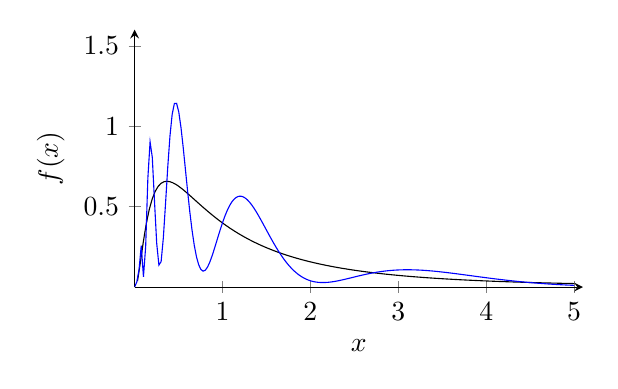
\begin{tikzpicture}
    \begin{axis}[
    axis lines=left,
    xlabel = $x$, ylabel = {$f(x)$},
    xmax = 5.1, xtick = {1, 2, 3, 4, 5},
    ymax = 1.6, ytick = {0.5, 1, 1.5},
    width=0.6\textwidth, height=0.4\textwidth]
    \addplot[domain=0:5, samples=150] {exp(-((ln(x))^2)/2)/(x*sqrt(2*pi))};
    \addplot[domain=0.001:5, samples=200, blue] {(1+0.8*sin(2*pi*(ln(\x)) r))*exp(-((ln(x))^2)/2)/(x*sqrt(2*pi))};
    \end{axis}
\end{tikzpicture}
\end{center}

We note that these two seemingly different random variables have the same $r$-th moment. To see this, it suffices to evaluate the integral
\begin{equation*}
    \int_0^\infty x^{r-1} \exp\bracket{-\frac{(\ln x)^2}{2}} \sin(2\pi \ln x) \, dx, \quad r = 0,1,...
\end{equation*}
With a variable substitution of $s = \ln x$ (such that $ds = dx/x$), the integral equals to 
\begin{equation*}
    \int_{-\infty}^\infty \exp\bracket{(r-1)s} \exp\bracket{-\frac{s^2}{2}} \sin(2\pi s) \, dx
\end{equation*}
Notice the integrand is an $L^1$ function multiplied by $\sin(2\pi s)$. Therefore,  by the Riemann-Lebesgue lemma, the integral is zero, and the two random variables have the same moments!
\end{example}

\begin{exercise}[Computing the moments of log-normal distribution] What happened? We can compute at the $r$-th moments of the log-normal distribution:
\begin{enumerate}
\item Verify that if $\xi$ has a standard normal distribution ($\mathsf{N}(0,1)$), then $\exp(\xi)$ has a standard log-normal distribution. 
\item Use LOTUS to compute the $r$-th moment being equal to $\exp(r^2/2)$.
\end{enumerate}
Notice that the moments grows too fast for the characteristic function to be analytical (i.e. possess a Taylor series)!
\end{exercise}

\subsection{Inversion Formula}
The main objective of this section is to make the inversion formula for characteristic functions precise. Let us state the first part of inversion formula.

\begin{theorem}[Inversion formula I] \label{thm:inversion_I}
Let $\mu$ be a probability measure on $(\R,\B(\R))$ with its corresponding distribution $F(x) = \mu((-\infty,x])$ and characteristic function $\varphi(t) = \int_\R e^{itx} \, \mu(dx)$. If $a<b$ then
\begin{equation}
\lim_{T\to\infty} \frac{1}{2\pi} \int_{-T}^T \frac{e^{-ita}-e^{-itb}}{it} \varphi(t) \, dt = \mu((a,b)) + \frac{\mu(\set{a}) + \mu(\set{b})}{2}
\end{equation}
In particular when $\mu(\set{a}) = \mu(\set{b}) = 0$, so that $F$ is continuous at $a,b$, then 
\begin{equation}
    F(b) - F(a) = \mu((a,b]) = \mu((a,b)) = \lim_{T \to \infty} \frac{1}{2\pi} \int_{-T}^T \frac{e^{-ita} - e^{-itb}}{it} \varphi(t) \, dt;
\end{equation}
\end{theorem}

Before we begin proving this theorem, let us recall some facts about the integral of the sinc function. Define
\begin{equation}
S(T) = \int_0^T \frac{\sin x}{x} \, dx.
\end{equation}

We note that $S(T)$ is a differentiable function with $S(T) > 0$ whenever $T > 0$, and that

\begin{lemma}
\begin{equation}
S(+\infty) = \int_0^\infty \frac{\sin x}{x} = \frac{\pi}{2}
\end{equation}
\end{lemma}

This can be proven by standard calculus tricks, either by differentiation under integral or residue calculus. \footnote{There is an entire article of teaching you how to integrate a since function! See \url{https://www.wikihow.com/Integrate-the-Sinc-Function}.} We therefore know that $S(T)$ is a bounded function and $\sup_{T>0} S(T)$ exists. \\

We also note the following scaling formula 
\begin{equation}
\int_0^T \frac{\sin(kx)}{x} \, dx= \int_0^T \frac{\sin(kx)}{kx} \, d(kx) = S(kT), \quad k > 0,
\end{equation}
and that when $k < 0$, we have
\begin{equation}
\int_0^T \frac{\sin(kx)}{x} \, dx= -\int_0^T \frac{\sin(|k|x)}{x} \, dx = -S(|k|T).
\end{equation}

In terms of the $\sgn$ function ($\sgn = \chi_{(0,\infty)} - \chi_{(-\infty,0)}$), we have for all $k \in \R$,
\begin{equation}
\int_0^T \frac{\sin(kx)}{x} = \sgn(k) S(|k|T).
\end{equation}

Finally, provided that the sinc function is even, we know that
\begin{equation}
\int_{-T}^T \frac{\sin(kx)}{x} = 2\sgn(k) S(|k|T).
\end{equation}

We are now ready to prove the first inversion formula:

\begin{proof} (of inversion formula I, theorem \ref{thm:inversion_I})
So let's first evaluate for fixed $T$,
\begin{equation}
I_T = \int_{-T}^T \frac{e^{-ita}-e^{-itb}}{it} \varphi(t) \, dt = \int_{-T}^T \int_\R \frac{e^{-ita}-e^{-itb}}{it} e^{itx} \, \mu(dx) \, dt
\end{equation}
We note that the integrand is bounded uniformly in $(t,x)$ (except when $t = 0$, which is a removable singularity):
\begin{equation}
\abs{\frac{e^{-ita} - e^{-itb}}{it} e^{itx}} \leq \abs{\int_a^b e^{-its} \, ds} \leq |b-a|, \label{eq:exponent_integral_estimate}
\end{equation}
so the integrand is integrable. By Fubini's theorem, we may exchange the order of integration:
\begin{equation}
I_T = \int_\R \int_{-T}^T \frac{e^{-ita}-e^{-itb}}{it} e^{itx} \, dt \, \mu(dx) = \int_\R \int_{-T}^T \frac{e^{it(x-a)}-e^{it(x-b)}}{it} \, dt \, \mu(dx) 
\end{equation}
We focus on the inner integral. Since the domain is now symmetric, we may ignore the odd parts of the integral, so we have
\begin{equation}
I_T = \int_\R \int_{-T}^T \frac{\sin(t(x-a)) - \sin(t(x-b))}{t} \, dt \, \mu(dx) 
\end{equation}
We have established a few facts about integrals on since function, and we want to utilise them here. To do so, we have to justify the following exchange the order of limits when evaluating $I_\infty$:
\begin{equation*}
I_\infty = \lim_{T\to\infty} I(T) \overset{(?)}{=} \int_\R \lim_{T\to\infty} \underbrace{\int_{-T}^T \frac{\sin(t(x-a)) - \sin(t(x-b))}{t}}_{J_{T,x}} \, dt \, \mu(dx) 
\end{equation*}
and here we will use dominated convergence theorem (DCT). Notice we have
\begin{equation*}
    \abs{J_{T,x}} \leq \abs{\int_{-T}^T \frac{\sin(t(x-a))}{t}} + \abs{\int_{-T}^T \frac{\sin(t(x-b))}{t}} \leq 4 \sup_{T>0} S(T) < \infty,
\end{equation*}
which is integrable with respect to the probability measure $\mu$. Therefore the condition for DCT is satisfied. \\

Let us now tabulate the values of $J_{\infty,x}$ for different values of $x$:
\begin{table}[h]
    \centering
    \begin{tabular}{c|c|c|c}
       $x$  & $\displaystyle{\int_{-\infty}^\infty \frac{\sin(t(x-a))}{t} \, dt }$ &  $\displaystyle{\int_{-\infty}^\infty \frac{\sin(t(x-b))}{t} \, dt}$ & $J_{\infty, x}$\\
       \hline
       $x>b$ & $\pi$ & $\pi$ & 0 \\
       $x=b$ & $\pi$ & 0 & $\pi$ \\
       $a<x<b$ & $\pi$ & $-\pi$ & $2\pi$ \\
       $x=a$ & $0$ & $-\pi$ & $\pi$ \\
       $x<a$ & $-\pi$ & $-\pi$ & 0
    \end{tabular}
\end{table}

and therefore we have 
\begin{equation*}
    I_\infty = \int_{\set{a}} \pi d\mu + \int_{\set{b}} \pi d\mu + \int_{(a,b)} 2\pi d\mu = 2\pi \bracket{\frac{\mu(\set{a}) + \mu(\set{b})}{2} + \mu((a,b))},
\end{equation*}

which completes the proof.
\end{proof}

Let us also state another inversion formula for obtaining the measures of an atom.

\begin{theorem}[Inversion formula II] \label{thm:inversion_II}
Under the setting of the first inversion formula (theorem \ref{thm:inversion_I}), we have
\begin{equation}
\mu(\set{a}) = \lim_{T\to\infty}\frac{1}{2T} \int_{-T}^T e^{-ita} \varphi(t) \, dt
\end{equation}
\end{theorem}

\begin{proof}
The proof is as similar as above, so we will only give a sketch. We first let 
\begin{align*}
I_T := \frac{1}{2T} \int_{-T}^T e^{-ita} \varphi(t) \, dt &= \frac{1}{2T} \int_{-T}^T \int_\R e^{it(x-a)} \, d\mu \, dt \\
&\overset{\text{(Fubini)}}{=} \int_\R \frac{1}{2T} \int_{-T}^T e^{it(x-a)} \, dt \, d\mu \\
&= \int_{\R} \frac{e^{iT(x-a)} -e^{-iT(x-a)}}{2iT(x-a)} \, d\mu \quad \text{see \footnote{when $x = a$ then let the integrated be 1 by continuity, but it doesn't really matter that much.}} \\
&= \int_{\R} \frac{\sin(T(x-a))}{T(x-a)} \, d\mu.
\end{align*}
We note that the integrand is uniformly bounded by one, which is integrable, so by DCT we have
\begin{equation}
I_\infty = \int_\R \bracket{\lim_{T\to\infty} \frac{\sin(T(x-a))}{T(x-a)} \, d\mu}.
\end{equation}
But note that the integrand tends to one when $x = a$ as $T \to \infty$ and zero otherwise, so we have
\begin{equation}
I_\infty = \lim_{T\to\infty}\frac{1}{2T} \int_{-T}^T e^{-ita} \varphi(t) \, dt = \mu(\set{a}). 
\end{equation}
\end{proof}

\begin{corollary} \label{cor:cf_dist_one_to_one}
Probability distributions on $(\R, \B(\R))$ and characteristic functions are in one-to-one correspondence.
\end{corollary}

\begin{proof}
So let's say $\mu,\nu$ are two measures on $(\R,\B(\R))$ such that they have the same characteristic function. By the inversion formulas we see that $\mu((a,b)) = \nu((a,b))$ for any $a<b$. Since the collection of open intervals $\set{(a,b) \,|\, a < b}$ generates $(\R,\B(\R))$, we must have $\mu = \nu$.
\end{proof}

The final inversion formula concerns the absolute continuity of a probability measure $\mu$ with respect to the Lebesgue measure (i.e. whether a continuous density exists). It turns out that if its characteristic function $\varphi$ is integrable, then we may invert the Fourier transform in the following sense

\begin{proposition}[Inversion formula III]
If $\int_{-\infty}^\infty |\varphi(t)| \d t < \infty$, then the probability measure $\mu(x)$ has density $f(x)$, in the sense that the distribution function $F$ satisfies
\begin{equation} \label{eq:density}
    F(x) = \mu((-\infty,x]) = \int_{-\infty}^x f(y) \, dy,
\end{equation}
and that the density is given by
\begin{equation} \label{eq:L1_inversion}
    f(x) = \frac{1}{2\pi} \int_{-\infty}^\infty e^{-itx} \varphi(t) dt.
\end{equation}
\end{proposition}

We note that this inversion formula coincides with the $L^1$ inversion formula for Fourier transform: let $f \in L^1(\R)$ and its Fourier transform (which is $\varphi(-t)$ with $\varphi$ being the characteristic function of the measure as defined in \eqref{eq:density}) is in $L^1$, then \eqref{eq:L1_inversion} holds with the minus sign replaced by a plus sign.

\begin{proof}
Utilise inversion formula I (theorem \ref{thm:inversion_I}) and the estimate \eqref{eq:exponent_integral_estimate}, we have
\begin{equation}
\mu((a,b)) + \frac{\mu(\set{a}) + \mu(\set{b})}{2} = \lim_{T\to\infty} \frac{1}{2\pi} \int_{-T}^T \frac{e^{-ita}-e^{-itb}}{it} \varphi(t) \leq \frac{b-a}{2} \int_\R |\varphi(t)| \, dt \lesssim \Leb((a,b)).
\end{equation}
This proves that $\mu \ll \Leb$, so that $\mu$ possess a density and has no atoms. We now prove that the function given in \eqref{eq:L1_inversion} is a density of $\mu$: note that
\begin{equation}
\mu((x,x+h)) = \frac{1}{2\pi} \int_\R \bracket{\int_x^{x+h} e^{-ity} \, dy} \, \phi(t) \, dt \overset{\text{(Fubini)}}{=} \int_x^{x+h} \bracket{\frac{1}{2\pi} \int_\R e^{-ity} \phi(t) \, dt} \, dy
\end{equation}
So $\mu$ has density function $f$ as given in \eqref{eq:L1_inversion}. It is easy to show that $f$ is continuous (by, e.g. dominated convergence theorem).
\end{proof}

\begin{exercise}
Show that the function $f$ as defined above is continuous by dominated convergence theorem.
\end{exercise}

We may use the third inversion formula to find the characteristic function for even more distributions.
\begin{exercise}
Let $\xi,\eta$ be a real-valued random variable.
\begin{enumerate}
    \item Find the characteristic function of $\xi$ if $\xi$ follows a triangular distribution with density
    \begin{equation}
        f(t) = (1-|x|)_+ := (1-|x|) \vee 0,
    \end{equation}
    then use the third inversion formula to show that the characteristic function of $\eta$ is $\varphi_\eta(t) = (1-|x|)_+$, where the $\eta$ follows a Polya's distribution \footnote{We follow the naming convention in \cite{Durrett}.} with density
    \begin{equation}
        f(t) = \frac{1-\cos x}{\pi x^2}.
    \end{equation}
    We will need this distribution to prove a theorem for the characterisation of characteristic function in section 6.4.
    \item Find the characteristic function of $\xi$ if $\xi$ follows a Laplace (bilateral exponential) distribution with density
    \begin{equation}
        f(x) = \exp(-|x|)/2,
    \end{equation}
    and hence find the characteristic function of $\eta$ if $\eta$ follows a Cauchy distribution with density
    \begin{equation}
        f(x) = (\pi(1+x^2))^{-1}.
    \end{equation}
\end{enumerate}
\end{exercise}

\subsection{Central Limit Theorem via Characteristic Functions}
We are almost able to prove the Central Limit Theorem. We need to prove the final (and the most important) step, the Levi's continuity theorem, which says if 

\begin{theorem}[Levi's Continuity theorem] \label{thm:levi_continuity}
Let $\varphi_n(t)$ be the characteristic functions of a sequence of probability measures $\p_n$ with on $(\R,\B(\R))$ distribution functions $F_n$. Then
\begin{enumerate}
    \item If $\p_n \to \p_\infty$ weakly, where $\p_\infty$ is a measure on $(\R,\B(\R))$, then $\varphi_n(t) \to \varphi_\infty(t)$ \textbf{pointwise} for all $t \in \R$, where $\varphi_\infty$ is the characteristic function of $\mu_\infty$.
    \item If $\lim_{n \to \infty} \varphi_n(t)$ exists $\forall t \in \R$, and $\varphi_\infty(t) = \lim_{n \to \infty} \varphi_n(t)$ is \textbf{continuous} at $t=0$, then $\varphi_\infty(t)$ is a characteristic function of some probability measure $\p$ and $\p_n \to \p$ (weakly). 
    \item If $\varphi_n(t)$ corresponds to $\p_n$ and $\varphi_\infty(t)$ is a characteristic function corresponding to $\p_\infty$, then
    \begin{equation*}
        \varphi_n(t) \to \varphi_\infty(t)\, \, \forall t \in R \iff \p_n \to \p_\infty \text{ (weakly)}.
    \end{equation*}
\end{enumerate}
\end{theorem}

We note that statement (1) is a direct consequence of the definition of weak convergence when applied to $\Re[e^{it\xi}]$, $\Im[e^{it\xi}]$.

\begin{unexaminable}
To prove statements 2 and 3, we need the following estimates:
\begin{lemma}
If $\p$ is a probability measure on $(\R,\B(\R))$ with characteristic function $\varphi(t)$, then for all $\epsilon > 0$, 
\begin{equation} \label{eq:cf_tail_bound}
    \p(\set{x \,|\, |x| \geq 2/\epsilon}) \leq \frac{1}{\epsilon} \int_{-\epsilon}^\epsilon (1-\varphi(t)) \, dt
\end{equation}
\end{lemma}

This lemma shows that the tail of measure $\p$, hence the existence of moments, is determined by the smoothness of $\varphi$ at zero. The direct connections between the existence of moments and smoothness are established in section 6.1.

\begin{proof}
First note that for all $x \neq 0$,
\begin{equation}
\int_{-\epsilon}^\epsilon (1-e^{itx}) \, dt = 2\epsilon - \frac{e^{it\epsilon} - e^{-it\epsilon}}{ix} = 2u\bracket{1-\frac{\sin \epsilon x}{\epsilon x}}
\end{equation}
We therefore have
\begin{align*}
    \frac{1}{\epsilon} \int_{-\epsilon}^\epsilon (1-\varphi(t)) \, dt 
    &= \frac{1}{\epsilon} \int_{-\epsilon}^\epsilon \bracket{1 - \int_\R e^{itx} \, \mu(dx)} \, dt \\
    &= \frac{1}{\epsilon} \int_{-\epsilon}^\epsilon \int_\R (1-e^{itx}) \, \mu(dx) \, dt \\
    &\overset{\text{(Fubini)}}{=} \int_\R \bracket{\frac{1}{\epsilon} \int_{-\epsilon}^\epsilon (1-e^{itx}) \, dt} \, \p(dx) \\
    &= \int_\R 2 \underbrace{\bracket{1 - \frac{\sin \epsilon x}{\epsilon x}}}_{\geq 0} \, \p(dx) \\ 
    &\geq 2 \int_{-2/\epsilon}^{2/\epsilon} \bracket{1 - \frac{\sin \epsilon x}{\epsilon x}} \, \p(dx) \\
    &\geq 2 \int_{-2/\epsilon}^{2/\epsilon} \underbrace{\bracket{1 - \frac{1}{|\epsilon x|}}}_{\geq 1/2} \, \p(dx) \\
    &\geq \p(\set{x \,|\, |x| \geq 2/\epsilon})
\end{align*}
\end{proof}

We are now ready to prove statements 2 and 3 of the continuity theorem.

\begin{proof}
We really only need to prove the second statement. When this is proven, the third statement follows from this and the inversion theorem. \\ 

\textbf{We first prove that the sequence $(\p_n)$ is tight.} We are given that $\varphi_\infty$ is continuous at 0 and that $\varphi_\infty(0) = 1$, so for all $\epsilon > 0$, there is $u > 0$ small enough that for all $t \in [-u,u]$, $1 - \varphi_\infty(t) \leq \epsilon / 4$, and hence 
\begin{equation}
\frac{\epsilon}{2} \geq \frac{1}{u} \int_{-u}^u (1-\varphi_\infty(t)) \, dt \overset{\text{(DCT)}}{=} \lim_{n\to\infty} \frac{1}{u} \int_{-u}^u \bracket{1-\varphi_n(t)} \, dt.
\end{equation}
As a result, there is $n_0$ such that for all $n \geq n_0$ such that 
\begin{equation}
\p_n\bracket{\R\setminus [-2/u,2/u]} \leq \frac{1}{u} \int_{-u}^u (1-\varphi_n(t)) \, dt \leq \epsilon
\end{equation}
We may choose smaller $u$ such that the above inequality holds for all $n \geq 1$, and hence we see that $(\p_n)_{n\geq 1}$ is tight. By Prokhorov theorem, for any subsequence of $(\mu_n)_{n\geq 1}$, say $(\mu_{n_k})_{k\geq 1}$, there is a further subsequence that converges weakly to the measure $\nu$. We note that by statement (1) of continuity theorem and uniqueness of limits we know that $\varphi_\infty(t)$ is the characteristic function of $\nu$, which also shows that the limiting measure must be unique regardless of what subsequence we have chosen. \\

We finally note that $\p_n \to \nu$ weakly, otherwise there is a point $y \in \R\setminus U_F$, $F$ distribution function of $\nu$, so that there is a subsequence $(\mu_{n'_k})_{k\geq 1}$ such that $|F_{n'_k}(y) - F(y)| \geq \epsilon$ for all $k$, but by above arguments there is a further subsequence $(\mu_{n_{k_j}})_{j\geq 1}$ which converges to $\nu$, which is a contradiction!
\end{proof}
\end{unexaminable}

Once we have the Levi's continuity theorem, we also have the following central limit theorems for free.

\begin{theorem}[Central Limit Theorem for Independent Identically Distributed Random Variables]
Let $\xi_1, \xi_2, \dots $ be a sequence of independent identically distributed (nondegenerate) random variables with $\E[\xi_1^2]] < \infty$ and $S_n = \xi_1 + \cdots + \xi_n$. Then as $n \to \infty$
\begin{equation*}
    \p \bigg\{ \frac{S_n - \E[S_n]}{\sqrt{\V[S_n]}} \le x \bigg\} \longrightarrow \Phi(x) \equiv \frac{1}{\sqrt{2\pi}} \int_{-\infty}^x e^{-u^2/2} \d u \quad \forall x \in \R.
\end{equation*}
\end{theorem}
\begin{remark}
The result can also be written as 
\begin{equation*}
    \frac{S_n - \E[S_n]}{\sqrt{\V[S_n]}} \xrightarrow{d} N(0,1).
\end{equation*}
\end{remark}
\begin{proof}
Set $m = \E[\xi_1]$, $\sigma^2 = \V[\xi_1]$, $\varphi(t) = \E[e^{it(\xi_1 - m)}]$.
If we put
\begin{equation*}
    \varphi_n(t) = \E\bigg[\exp \bigg(it \frac{S_n - \E[S_n]}{\sqrt{\V[S_n]}} \bigg)\bigg],
\end{equation*}
by independence 
\begin{equation*}
    \varphi_n(t) = \bigg[\varphi\bigg(\frac{t}{\sigma \sqrt{n}}\bigg)\bigg]^n.
\end{equation*}
Since $\E[\xi_1^2] < \infty$, we have by properties of characteristic functions (theorem above) that 
\begin{equation*}
    \varphi(t) = 1 - \frac{\sigma^2 t^2}{2} + o(t^2), \quad t \to 0.
\end{equation*}
So $\varphi_n(t) = [1 - t^2/(2n) + o(1/n)]^n \to e^{-t^2/2}$ for all $t \in \R$. This is the characteristic function of $\mathsf{N}(0,1)$ and so the result follows by continuity theorem.
\end{proof}
\begin{theorem}[Central Limit Theorem for Independent Random Variables]
Let $\xi_1, \xi_2, \dots$ be a sequence of independent random variables with finite second moments $\E[\xi_j] < \infty$ and distribution functions $F_j$ for all $j$. Let $$m_j = \E[\xi_j], \sigma_j^2 = \V[\xi_j] >0,\quad S_n = \xi_1 + \cdots + \xi_n \text{ and } D_n^2 = \sum_{j=1}^n \sigma_j^2.$$ 
Suppose that the Lindeberg condition is satisfied: for every $\varepsilon > 0$
\begin{equation*}
    \frac{1}{D_n^2}\sum_{k=1}^n \int_{\{x:|x-m_k|\ge \varepsilon D_n \}} (x-m_k)^2 \d F_k(x) \to 0, \quad n \to \infty.
\end{equation*}
Then 
\begin{equation*}
    \frac{S_n - \E[S_n]}{\sqrt{\V[S_n]}} \xrightarrow{d} N(0,1).
\end{equation*}
\end{theorem}
We turn our attention to some special cases in which the Lindeberg condition is satisfied and consequently, the central limit theorem is valid.
\begin{itemize}
    \item Let the \textit{Lyapunov condition} be satisifed: for some $\delta > 0$
    \begin{equation*}
        \frac{1}{D_n^{2 +\delta}} \sum_{k=1}^n \E[|\xi_k - m_k|^{2+\delta}] \to 0 \quad n \to \infty.
    \end{equation*}
    Let $\varepsilon > 0$. Then
    \begin{align*}
        \E[|\xi_k - m|^{2+\delta}] &= \int_{-\infty}^\infty |x - m_k|^{2+\delta} \d F_k(x)\\
        &\ge \int_{\{x: x|x-m_k| \ge \varepsilon D_n\}} |x - m_k|^{2+\delta}  \d F_k(x)\\
        &\ge \varepsilon^\delta D_n^\delta \int_{\{x: |x-m_k| \ge \varepsilon D_n\}} (x - m_k)^{2}  \d F_k(x),
    \end{align*}
    and therefore 
    \begin{equation*}
        \frac{1}{D_n^2}\sum_{k=1}^n \int_{\{x: |x-m_k| \ge \varepsilon D_n\}} (x - m_k)^{2}  \d F_k(x) \le \frac{1}{\varepsilon^\delta} \frac{1}{D_n^{2 + \delta}} \sum_{k=1}^n \E[|\xi_k - m_k|^{2 + \delta}].
    \end{equation*}
    Consequently, the Lyapunov condition implies the Lindeberg condition.
    \item Suppose that there exists $K$ such that for all $n \ge 1$
    \begin{equation*}
        |\xi_k| \le K < \infty, \quad \forall k,
    \end{equation*}
    where $D_n \to \infty$ as $n \to \infty$. This condition also implies Lindeberg condition (exercise).
\end{itemize}
\begin{theorem}[Berry-Esseen Inequality]
Let $\xi_1, \xi_2, \dots$ be a sequence of independent and identically distributed random variables with $\E[|\xi_1|^3] < \infty$. Then
\begin{equation*}
    \sup_x \bigg| \p\bigg( \frac{S_n - \E[S_n]}{\sqrt{\V[S_n]}} \le x\bigg) - \Phi(x) \bigg| \le C\frac{\E[|\xi_1 - \E[\xi_1]|^3]}{\sigma^3\sqrt{n}},
\end{equation*}
where the absolute constant $C$ satisfies the inequality
\begin{equation*}
    \frac{1}{\sqrt{2\pi}} \le C < 0.8.
\end{equation*}
\end{theorem}
\begin{remark}
$O(1/\sqrt{n})$ is optimal. Indeed, let $\xi_1, \xi_2, \dots$ be independent and identically distributed Bernoulli random variables, 
\begin{equation*}
    \p(\xi_k = 1) = \p(\xi_k = -1) = \frac12.
\end{equation*}
Then by symmetry,
\begin{equation*}
    2\p\bigg(\sum_{k=1}^{2n} \xi_k < 0\bigg) + \p\bigg(\sum_{k=1}^{2n} \xi_k = 0\bigg) = 1
\end{equation*}
and therefore,
\begin{equation*}
    \bigg|\p\bigg(\sum_{k=1}^{2n} \xi_k < 0\bigg) - \frac12 \bigg| = \frac12 \p\bigg(\sum_{k=1}^{2n} \xi_k = 0\bigg) = \frac12 \binom{2n}{n} \frac{1}{2^{2n}} \sim \frac{1}{2\sqrt{\pi n}} = \frac{1}{\sqrt{2\pi}\sqrt{2n}}.
\end{equation*}
Then $\E[|\xi_1|^3] = 1 = \sigma_1$, so the theorem cannot be improved in terms of $O(1/\sqrt{n})$ and $C \ge \frac{1}{\sqrt{2\pi}}$.
\end{remark}

\begin{example}[Cauchy Distribution]
What happens if $\E[\xi^2] = \infty$? Let $\xi_1, \xi_2, \dots$ be i.i.d. with Cauchy distribution, i.e. with density
\begin{equation*}
    f = \frac{\theta}{\pi(x^2 + \theta^2)}, \quad \theta>0.
\end{equation*}
Then 
\begin{equation*}
    \varphi_{\xi_1}(t) = \frac{\theta}{\pi} \int_{-\infty}^\infty  \frac{e^{itx}}{x^2 + \theta^2}\d x = e^{-t\theta}, \, \,t>0
\end{equation*}
and similarly for $t < 0$. So
\begin{equation*}
    \varphi_{\xi_1}(t) = e^{-\theta |t|}, t \in \R,
\end{equation*}
which implies that 
\begin{equation*}
    \varphi_{S_n/n} (t) = (e^{-\theta|t|/n})^n = e^{-\theta|t|},
\end{equation*}
and thus $S_n/n$ also has the Cauchy distribution!
\end{example}

\begin{exercise}
Verify the characteristic function for the above (standard) Cauchy distribution.
\end{exercise}

\subsection{More about constructing characteristic function}
\textcolor{red}{This section will be finished in the later edition.}
\begin{theorem}[Bochner-Khinchin]
Let $\varphi(t)$ be continuous, $t\in \R$, with $\varphi(0) = 1$. A necessary and sufficient condition that $\varphi(t)$ is a characteristic function is that it is positive semi-definite, i.e. that for all real $t_1, \dots, t_n$ and all complex $\lambda_1, \dots, \lambda_n$, $n=1,2,\dots$,
\begin{equation*}
    \sum_{j,k = 1}^n \varphi(t_j - t_k)\lambda_j \overline{\lambda}_k \ge 0.
\end{equation*}
\end{theorem}
\begin{theorem}[Polya's Theorem]
Let a continuous even function $\varphi(t)$ satisfy $\varphi(t) \ge 0$, $\varphi(0) = 1$, $\varphi(t) \to 0$ as $t \to \infty$ and let $\varphi(t)$ be convex on $0 \le t < \infty$ (hence also on $(0, \infty)$). Then $\varphi(t)$ is a characteristic function.
\end{theorem}
\begin{unexaminable}
\begin{proof}
\red{Sketch of proof needed. (Not necessary full proof).}
\end{proof}
\end{unexaminable}
This theorem provides a very convenient method of constructing characteristic functions. Examples are
\begin{align*}
    \varphi_1(t) &= e^{-|t|}\\
    \varphi_2(t) &= \begin{cases}
    1 - |t| & |t| \le 1,\\
    0 & |t| > 1.
    \end{cases}
\end{align*}
Another is the function $\varphi_3(t)$ drawn below. On $[-a, a]$, as, the function $\varphi_3(t)$ coincides with $\varphi_2(t)$. However, the corresponding distribution functions $F_2$ and $F_3$ are evidently different.

\begin{center}
\includegraphics[scale=0.7]{figures/charact_functions.png}
\end{center}

This example shows that in general two characteristic functions can be the same on a finite interval without their distribution functions being
the same.

\begin{theorem}[Marcinkiewicz's Theorem]
If a characteristic function $\varphi(t)$ is of the form $e^{p(t)}$, where $p(t)$ is a polynomial, then this polynomial is of degree at most $2$.
\end{theorem}
It follows, for example, that $e^{-t^4}$ is not a characteristic function. 

\begin{proof}
\red{Sketch of proof needed. (Not necessary full proof). In particular, what's wrong with the function $e^{-t^4}$?}
\end{proof}

\subsection{Cumulants}
\begin{definition}
If there exists expansion 
\begin{equation*}
    \log \varphi_\xi(t) = \sum_{k=0}^n \frac{(it)^k}{k!} s_k + o(|t|^n), \quad t \to 0,
\end{equation*}
then the coefficients $s_k$ are called \textbf{cumulants} of $\xi$.
\end{definition}
\begin{exercise}
Show that 
\begin{equation*}
    \E[\xi] = s_1, \quad \V[\xi] = s_2.
\end{equation*}
\end{exercise}

\red{What is $s_3$, $s_4$ and so on? Turns out there is a connection between cumulants and moments via counting the total possible non-crossing partitions. This is a fundamental ingredient of non-commutative (free) probability. I may try to include a sketch of arguments here.}

\begin{remark}
\begin{itemize}
    \item[]
    \item If $\xi \sim N(m, \sigma^2)$ then
    \begin{equation*}
        s_1 = m, \quad s_2 = \sigma^2, \quad s_k = 0, \quad k\ge3.
    \end{equation*}
    \item In general, by Marcinkiewsicz's Theorem if for a random variable $\xi$ there exists $n$ such that $s_k = 0,$ for all $k \ge n$, then also $s_k = 0$ for all $k \ge 3$ and $\xi \sim N(s_1, s_2)$.
\end{itemize}
\end{remark}
The following theorem shows that a property of the characteristic function of a random variable can lead to a non-trivial conclusion about the nature of the random variable
\begin{theorem}
Let $\varphi(t)$ be a characteristic function of $\xi$.
\begin{enumerate}
    \item If $|\varphi(t_0)| = 1$ for some $t_0 \ne 0$, then $\xi$ is concentrated at the points $a + nh$, $h = 2\pi/t_0$, for some $a$, that is,
    \begin{equation*}
        \sum_{-\infty}^\infty \p(\xi = a + n h) = 1,
    \end{equation*}
    where $a$ is a constant.
    \item If $|\varphi(t)| = |\varphi(\alpha t)| = 1$ for two different points $t$ and $\alpha t$, where $\alpha$ is irrational, then $\xi$ is degenerate, that is 
    \begin{equation*}
        \p(\xi = a) = 1,
    \end{equation*}
    where $a$ is some constant.
    \item If $|\varphi(t)|\equiv 1$, then $\xi$ is degenerate.
\end{enumerate}
\end{theorem}
\begin{proof}
\begin{enumerate}
    \item If $|\varphi(t_0)| = 1$, $t_0 \ne 0$, there is a number $a$ such that $\varphi(t_0) = e^{i t_0 a}$. Then
    \begin{align*}
        e^{i t_0 a} &= \int_{-\infty}^\infty e^{i t_0 x} \d \, F(x) \implies 1 = \int_{-\infty}^\infty e^{i t_0 (x-a)} \d \, F(x) \implies \\
        1 &= \int_{-\infty}^\infty \cos{ t_0 (x-a)} \d \, F(x) \implies \int_{-\infty}^\infty 1 - \cos{ t_0 (x-a)} \d \, F(x) = 0.
    \end{align*}
    Since $1 - \cos{t_0(x-a)} \ge 0$, it follows that 
    \begin{equation*}
        1 = \cos t_0(x-a) \quad (\p\text{-a.s.}).
    \end{equation*}
    \item If follows from $|\varphi(t)| = |\varphi(\alpha t)| = 1$ and from the previous statement that
    \begin{equation*}
        \sum_{n=-\infty}^{\infty} \p(\xi = a + \frac{2\pi}{t}n) = \sum_{m=-\infty}^{\infty} \p(\xi = b + \frac{2\pi}{\alpha t} m) = 1.
    \end{equation*}
    If $\xi$ is not degenerate, then there must be at least two common points:
    \begin{equation*}
        a + \frac{2\pi}{t} n_1 = b + \frac{2\pi}{ \alpha t} m_1, \quad a + \frac{2\pi}{t} n_2 = b + \frac{2\pi}{ \alpha t} m_2,
    \end{equation*}
    in the sets 
    \begin{equation*}
        \bigg\{ a + \frac{2\pi}{t}n, n=0, \pm 1, \dots \bigg\} \quad \text{and} \quad \bigg\{ b + \frac{2\pi}{\alpha t}m, m=0, \pm 1, \dots \bigg\},
    \end{equation*}
    whence 
    \begin{equation*}
        \frac{2\pi}{t}(n_1 - n_2) = \frac{2\pi}{\alpha t} (m_1 - m_2),
    \end{equation*}
    and this contradicts the assumption that $\alpha$ is irrational. Conclusion $3.$ follows from $2.$
\end{enumerate}
\end{proof}
\begin{exercise}
\begin{enumerate}
    \item[]
    \item Let $\varphi(t)$ be a characteristic function. Show that the following are also characteristic functions:
    \begin{equation*}
        |\varphi(t)|^2, \quad e^{\lambda(\varphi(t) - 1)}, \quad \lambda \ge 0, \quad \int_0^1 \varphi(u t) \d u, \quad  \int_0^\infty e^{-u} \varphi(u t) \d u
    \end{equation*}
    \item Let $X$ and $Y$ be independent identically distributed random variables with zero mean and unit variance. Prove using characteristic functions that if the distribution $F$ of $(X+Y)/\sqrt{2}$ is the same as that of $X$ and $Y$, then $F$ is the normal distribution.
    \item Let $\xi$ be an integer-valued random variable and $\varphi_\xi(t)$ be its characteristic function. Show that
    \begin{equation*}
        \p(\xi = k) = \frac{1}{2\pi} \int_{-\pi}^\pi e^{-ikt} \varphi_\xi(t) \d t, \quad k = 0, \pm 1, \pm 2, \dots
    \end{equation*}
    \item Let $\varphi_k(t)$, $k=1,2,\dots,n$ be characteristic functions and let the nonnegative numbers $\lambda_k$ satisfy $\sum_{k=1}^n \lambda_k = 1$. Show that 
    \begin{equation*}
        \sum_{k=1}^n \lambda_k \varphi_k(t)
    \end{equation*}
    is a characteristic function.
    \item Show that if $\varphi(t)$ is a characteristic function, then $\Re[\varphi(t)]$ is also a characteristic function, but $\Im[\varphi(t)]$ is not.
\end{enumerate}
\end{exercise}
\newpage